\documentclass[a4wide]{article}
\usepackage{a4wide}
\usepackage{graphicx}
\usepackage{appendix}
\usepackage{hyperref}
\newcommand{\comment}[1]{{\tt #1}}

\title{RocketMouse:\\ System Requirements Specification}

\author{Hesham H. Salman \and Jonathan Kissinger \and Sean Mead
\and Troy Johnson}

\begin{document}
\maketitle

\section{Introduction}

\subsection{Overall Description}
\indent RocketMouse tracks the user inputs and behavioral patterns of a user playing a mobile game, and uses this data to
determine whether or not the user is likely to have ADHD. This is determined by
comparing the user response times and input patterns to those of people with and
without ADHD. If the application can determine with a high level of confidence
that the user is likely to have ADHD, a suggestion is made to the user to visit
a medical professional. \par
This application is designed to be used by a number of people with and without ADHD so that we may test it's detection algorithms and the accuracy of those ADHD detection algorithms.


\subsection{Overview of Developer's Responsibilities}

The developer is responsible for development and deployment of the RocketMouse
application to iOS systems. The developer is responsible for the maintenance
of the system with regards to new feature development and bug fixes. The developer is also responsible for looking for new trends in the data that may be able to point towards new indications of somebody who has ADHD.

%%%%%%%%%%%%%%%%%%%%%%%%%%%%%%%%%%%%%%%%%%%%%%%%%%%%%%%%%%%%%%%%%%%%%%%%%%%

\section{System Overview}

\subsection{Survey}

The user survey is loaded during the applications's initial launch screen.
The user is responsible for filling out the questions to the best of their ability in order to receive as accurate results as possible.
The survey will be submitted and uploaded to the server upon completion. 

\subsection{Server}

The server is responsible for accepting user submission information and introducing it to the database.
Communication between the server and clients will be encrypted and as secure as possible to protect any sensitive information. The server is also responsible for parsing the uploading data, processing it, and coming up with some kind of feedback for the user, if enough data has already been previously submitted.

%%%%%%%%%%%%%%%%%%%%%%%%%%%%%%%%%%%%%%%%%%%%%%%%%%%%%%%%%%%%%%%%%%%%%%%%%%%

\section{General Description}

\subsection{Product Perspective}

RocketMouse is a game that collects the user's response times and usage metrics.
The information collected is stored in a local database, anonymized, and sent to
a remote server for data processing. The data processing feeds information for
calibration of a model that aims to predict the likelihood of a user having ADHD.

\subsection{Product Functions Overview}

\begin{enumerate}
\item Game Functionality: RocketMouse
\item User input tracking and data collection
\item Data processing to determine whether or not the user has ADHD
\item Result generation
\item Comparative analysis of user's data with average user data
\end{enumerate}

\subsection{User Characteristics}

The users of this application are to be people with and without ADHD. A user
survey is conducted at the start of this application such that the results can
be calibrated based on the user's age and gender. Of users with ADHD, there is a
distinction made between users that are medicated and unmedicated.

\subsection{General Constraints}

This project is to be completed to the extent that some data has been collected by
November 30, 2014. Once data has been collected, a model can be created from the
information gathered and a test of the model can be conducted.

%%%%%%%%%%%%%%%%%%%%%%%%%%%%%%%%%%%%%%%%%%%%%%%%%%%%%%%%%%%%%%%%%%%%%%%%%%%

\section{Functional Requirements}

\begin{enumerate}
\item Introductory User Survey
\item Home Screen
\item Volume Control
\item Data Collection
\item Data Encryption
\item Game Functionality
\item Data transfer and processing
\item Result display
\end{enumerate}


\subsection{Introductory User Survey}
The introductory user survey is displayed on the first load of the mobile application. It must
be completed before the home screen is allowed to display and the user allowed to play the game. The introductory user
survey establishes information to better understand the user's state, this includes: whether or
not they have been diagnosed with ADHD (and if they have, whether or not they
are currently taking medicine), their age, and their gender. This information is
required so that the calculations regarding the likelihood of ADHD are accurate.
In the case that the user does not complete the survey, their incomplete
survey state is saved, and will be loaded upon re-launch of the program.

\subsection{Home Screen}
The home screen must display two navigation options to the user: the option to
begin the game and the option to enter the settings pane. In the case that the
user does not select an option, the program will remain in the home-screen
state.

\subsection{Volume Control}
Allows the user to toggle audio volume.

\subsection{Data Collection}
Collects the following usage metrics from the user:
\begin{enumerate}
\item Introductory User Survey
\item Reaction Time
\item Amount Played
\item Number of encounters
\item Average Session Length
\end{enumerate}

Furthermore, error logs are collected in the event of an error. All data is
logged in a local database and tagged with a unique identifier.

\subsection{Data Encryption}
The data is encrypted with an RSA encryption scheme because survey results and
collected data may be sensitive.

\subsection{Game Functionality}
The game involves a single character sprite running rightwards, avoiding
obstacles which appear at pseudo-random intervals.

\subsection{Data Transfer and Processing}
The data is transferred to a remote server where it is processed. The processing
involves statistical normalization of the information, as well as comparison
with our model. Once the data is transferred to the server, the model determines
whether or not the user's individual data follows the same correlative trends as
those users with ADHD.

\subsection{Result Display}
Two results must be displayed to the user:
\begin{enumerate}
\item The Game Score
\item Their likelihood of having ADHD
\end{enumerate}
The game score is calculated as the result of the game, whereas their likelihood
of having ADHD must be processed remotely and transferred back to the user.

\section{Non-functional Requirements}
\begin{itemize}
\item Easily understandable -- the software should be easy to use and understand
\item Entertaining -- the game must be entertaining to the users so as to
encourage usage
\item Enhanceable -- the system must allow for enhancement without major code
rewrites or architectural changes; coupling must be limited
\item Reusable -- the components of the system should be reusable
\item Stable -- the system must be stable on all target versions of iOS 8.0 or greater
\item Good performance -- the system should provide good performance on all
targeted platforms
\item Responsive -- the system should respond to user actions immediately.
\item Clean interface -- the interface should be simple and clean so as to not
confuse users.
\end{itemize}

%%%%%%%%%%%%%%%%%%%%%%%%%%%%%%%%%%%%%%%%%%%%%%%%%%%%%%%%%%%%%%%%%%%%%%%%%%%

\section{External Interface Requirements}

\subsection{User Interfaces}

The application will use the touchscreen interface of the mobile device it is
installed on.  The primary function will be tapping the screen to jump.
Secondary functions include navigating the included survey and any menus that may
be necessary to include.

\subsection{Hardware Interfaces}

Mobile device running a compatible version of the iOS operating system that is greater than or equal to 8.0.


\subsection{Software Interfaces}

iOS versions, including version 8.0 and above.


%%%%%%%%%%%%%%%%%%%%%%%%%%%%%%%%%%%%%%%%%%%%%%%%%%%%%%%%%%%%%%%%%%%%%%%%%%%

\section{Performance Description}

\subsection{Response Time}
As this application is measuring user reaction time, the response time will need
to be as minimal as possible to allow more precise measurements.  Human reaction
time has a limit of about 180 milliseconds.  Our application should have a
response time less than 100 milliseconds to be effective.

\subsection{Processing Time}
This follows the same constraints as above.  Processing of user input needs to
be near instantaneous.  Data that is collected may be transmitted to the
database for storage when convenient, for example between games, such that it
does not affect the processing of the application.

\subsection{Memory Constraints}
Memory constraints will be minimal due to the nature of the application.
However, this should be verified as the application is intended to be used on
mobile devices which have severe constraints to both processing and memory.

\subsection{Security \& Privacy}
Because of the sensitive nature of some of the data collected, the application
must be secure and must not store any data locally.  One possible exception is
the circumstance when there are multiple users on the same device.  In this case,
an anonymous identifier will be generated locally to differentiate between
users.  Data must be transmitted to a secure database from memory and never
stored on disk.

\subsection{Storage Requirements}
A secure database must be present for receiving data transmitted by the
application.  The database must be capable of handling transmissions from
multiple users at once.  There must also be sufficient space.  At a minimum we
would expect 50-100 users, and depending on the popularity of the application,
as many as a few hundred.


%%%%%%%%%%%%%%%%%%%%%%%%%%%%%%%%%%%%%%%%%%%%%%%%%%%%%%%%%%%%%%%%%%%%%%%%%%%

\section{Exception Handling}

\subsection{Form}

In general user forms are prone to exceptions.
Handling these exceptions is crucial to valid form submission.
Each field will be appropriately handled and validated before submission.

\subsection{Network}

Network communication may fail from either the client or server end.
In these cases proper exception handling is important.
The code must be versatile enough to put up with null or delayed responses.


%%%%%%%%%%%%%%%%%%%%%%%%%%%%%%%%%%%%%%%%%%%%%%%%%%%%%%%%%%%%%%%%%%%%%%%%%%%

\section{Design Constraints}

\subsection{Standards Compliance}

Must be iOS Compliant, as defined in [1]. [1] also provides the complete process for uploading a mobile application to the iTunes store, submitting apps for review, and pretty much anything else associated with submitting a mobile iOS application to iTunes.

\subsection{Hardware Limitations}

This application is only targeted at iOS devices running version 8.0 or 
higher. The device must have networking capability in order to upload data for processing and to receive the results of the data processing.

%%%%%%%%%%%%%%%%%%%%%%%%%%%%%%%%%%%%%%%%%%%%%%%%%%%%%%%%%%%%%%%%%%%%%%%%%%%


\section{Validation Criteria}

\subsection{Documentation}
The software for both the client side mobile application must be fully
documented and clearly readable. The documentation should adequately describe
what is occurring within the code in a clear and concise manner. The code should
also be as loosely coupled as possible to allow desirable changes to be easily
made to the code and to also reduce the possibility of errors cropping up when
a developer wants to make changes to the code base. This is important, especially
on the server side, as the algorithm for determining the possibility of ADHD may
be constantly changing and refined over time as more and more data becomes
available and new patterns in the data are picked up on that may help diagnose a
user with ADHD.
\subsection{Testing}
The mobile application must be able to be run on a variety of iOS operating
systems. Ideally, the application will run on all iOS versions greater than
or equal to iOS 8.0. The application should pass all 
tests we develop using NUnit to test the application for possible errors on the 
mobile application side along with server passing all stress tests performed on 
it. If these tests are passed, and the user can successfully upload their data and
get results back (if enough data is available), then the mobile application will 
pass its acceptance criteria as a prototype for an application with the potential 
for helping to diagnose users with ADHD.


%%%%%%%%%%%%%%%%%%%%%%%%%%%%%%%%%%%%%%%%%%%%%%%%%%%%%%%%%%%%%%%%%%%%%%%%%%%

\newpage
\appendix
\appendixpage

\section{References}
[1]Apple Inc. "ITunes Connect Developer Guide." : Submitting the App to App Review. Apple Inc, 24 Oct. 2014. Web. 27 Oct. 2014.

\begin{description}
\item[Interviewee] Dr. Tony Morelli
\item[Position] Professor of Computer Science
\item[Affiliation] Central Michigan University
\item[Interviewer] Jonathan Kissinger
\item[Date] Thursday, 9/18/2014
\item[Start Time] 2:00pm
\item[End Time] 2:30pm
\end{description}
\textbf{Q. We're considering using Unity for our game engine, but we would need
access to Unity Pro to run native android code.  Does the school grant access to
that software and is it appropriate for our needs?}\\
A. Yes, the school has Unity Pro on the lab computers in PE 400.  It may also be
available on the Virtual Machines accessible remotely.  However, Unity may be a
bit more than what you need.  You're aware of the project I recently did with
interface testing and Unity and it worked well for that but it's really up to
you.\vspace{2.0 mm}\\
\textbf{Q. In your research you used ISO standards, are there any applicable to
reaction time and our project?}\\
More than likely, check out ISO 9241 it contains most standards like that.  It's
primarily aimed at interfaces but there are lots of other standards contained
within it.\vspace{2.0 mm}\\
\textbf{Q. We need to file an IRB application to have anonymous surveys and data
collection right?}\\
Yes, the best thing to do is give them a call.  They'll tell you which form to
fill out and send in.  I had to fill out 3 different forms last time because I
kept filling out the wrong one.  You'll need a professor to sponsor the project,
which I will be glad to do if Dr. Lee doesn't wish to.\vspace{2.0 mm}\\
\textbf{Q. Is it possible to save the interviewing step and submit a prototype
for publication?}\\
Yes, that would be called a work in progress and it's something that's not
uncommon.  They get accepted for publication just like regular papers.

\section{Functional Model}
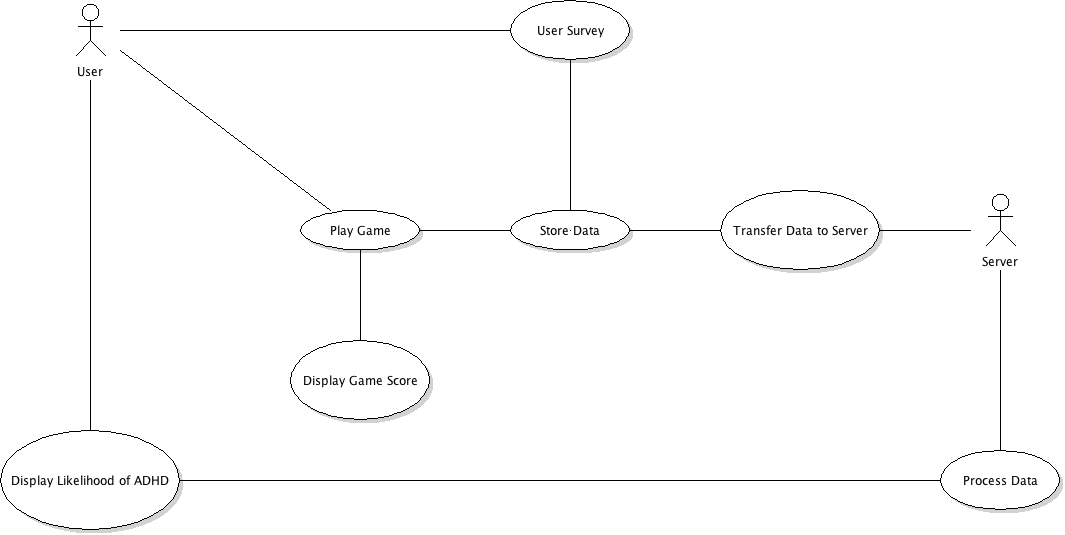
\includegraphics[width=\textwidth]{images/UseCaseDiagram.png}
\small Fig. 1: Use Case Diagram involving user and server actions
\section{State Diagram}
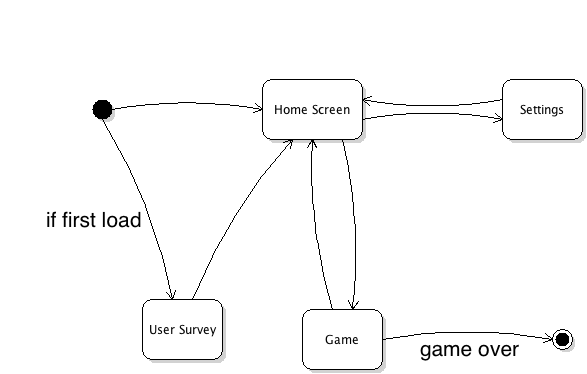
\includegraphics[width=\textwidth]{images/StateDiagram.png}
Fig. 2: State Diagram for RocketMouse

\section{Dynamic Model}
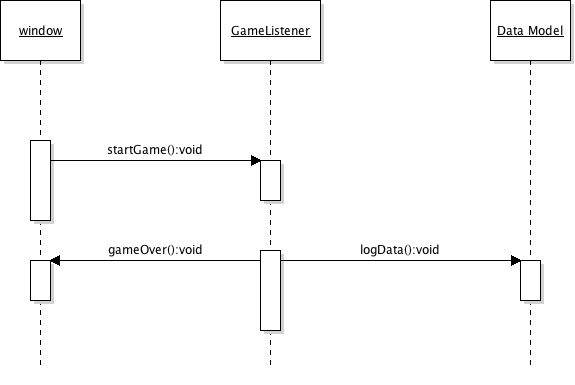
\includegraphics[width=\textwidth]{images/dynamicModel.png}
Fig. 3: Dynamic Model for RocketMouse

\section{Gantt Chart}
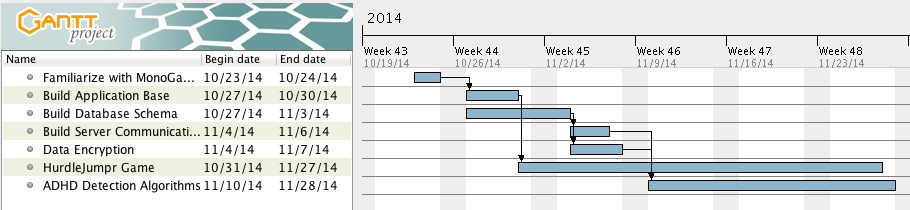
\includegraphics[width=\textwidth]{images/Gantt.png}
Fig. 4: Gantt Chart




\end{document}
